\documentclass[../../master.tex]{subfiles}
\begin{document}
\chapter{Design}\label{ch:design}
The aim of this chapter is to design the architecture components which will eventually guide the implementation of the system.

This chapter is divided into the following parts: Architecture Design, Application Method, and Component Design.
The Architecture Design in \cref{sec:architecturedesign} will introduce and discuss the criteria and the requirement priorities.
In the Application Method section, the main framework that the system will be implemented within is introduced and discussed.
In Component Design in \cref{sec:componentdesign}, the theory for component design will be introduced, followed by the project's architecture component design.

\subfile{Chapters/Design/ArchitectureDesign.tex}
\subfile{Chapters/Design/application.tex}
\section{Component Design} \label{sec:componentdesign}

In this section the component design theory will be introduced and elaborated.
This theory will be utilized in the following section where the component design for the system will be presented.
%Anna: evt fjerne sætningen ovenfor da det virker til at være en gentagelse af den første

\subsection{Components}


\subsection{System design} \label{sec:systemdesign}

In relation to the ASP.NET MVC pattern there are immediate similarities to the component design theory in \cref{archicomponents}.
There can among other be drawn parallels between the \textit{model} component and the \textit{model} classes in the MVC pattern.
The possible parallels are listed in the table below.

\begin{table}
	\centering
	\begin{tabular}{| c | c | }
	\hline
	\textbf{Components} & \textbf{MVC Pattern} \\
	\hline
	Model & Model \& EF Core \\
	\hline
	Functionality & Controller \\
	\hline
	Interface & View \\
	\hline
\end{tabular}
\caption{{\color{red}indsæt caption tekst}}\label{tab:PatternParallels}
\end{table}

As written in the component design theory in \cref{sec:archicomponents} the model components should seek to solve the problem of the problem domain.
%Anna: enten henvis til specifikke definition hvis sådan en eksisterer ellers henvis til afsnittet.
%Anna: Mener vi virkeligt "problem og the problem domain"
The model component in the MVC pattern is likewise going to contain the classes and objects that seeks to solve the problem domain through meeting the requirements written in {\color{red}section xx}.
The model component in the implementation is among other classes going to contain \textit{documents, users, departments, versions, approvals} and \textit{read statuses}.
The arguments for including these classes can be seen in \cref{sec:classdiagram}.
The database in form of EF Core is also included in the model component as this in part also seeks to solve the problem domain.
%Anna: Vi hrar endnu ikke introdyuceret denne forkortelse i brødteksten(EF core)

As written in the component design theory the responsibilty of the functionality is to provide the actor a means to access the model component.
%Anna: Henvis til afsnitet
%Anja: Der er blevet henvist i paragraffen ovenfor. Det begynder at blive overkill
The controller component in the MVC pattern does this by communicating between the model component and the view component.
The controllers retrieves data from the database and both methods and objects from the models.
Hereafter,it links these to the view.

The responsibility of the interface component is the handle the interaction between the users and the functionality.
This is done through the view model in the MVC pattern as the interface is handled in big part due to HTML, CSS and JavaScript.
These are what determines what the actors sees and what they can interact with.

\subsection{Component layers}
In relation to the theory written in \cref{archicomponents} the components can be designed in layers to describe their responsibilities and relation to each other.
The components in the MVC pattern with EF Core included can also be designed with the layered architecture in mind.
To give an overview and understanding of the architecture and design a simple component layer design can be seen in the figure below:
%Anna: synes den sidste sætning bliver en smule kringlet

\begin{figure}[H]
	\centering
	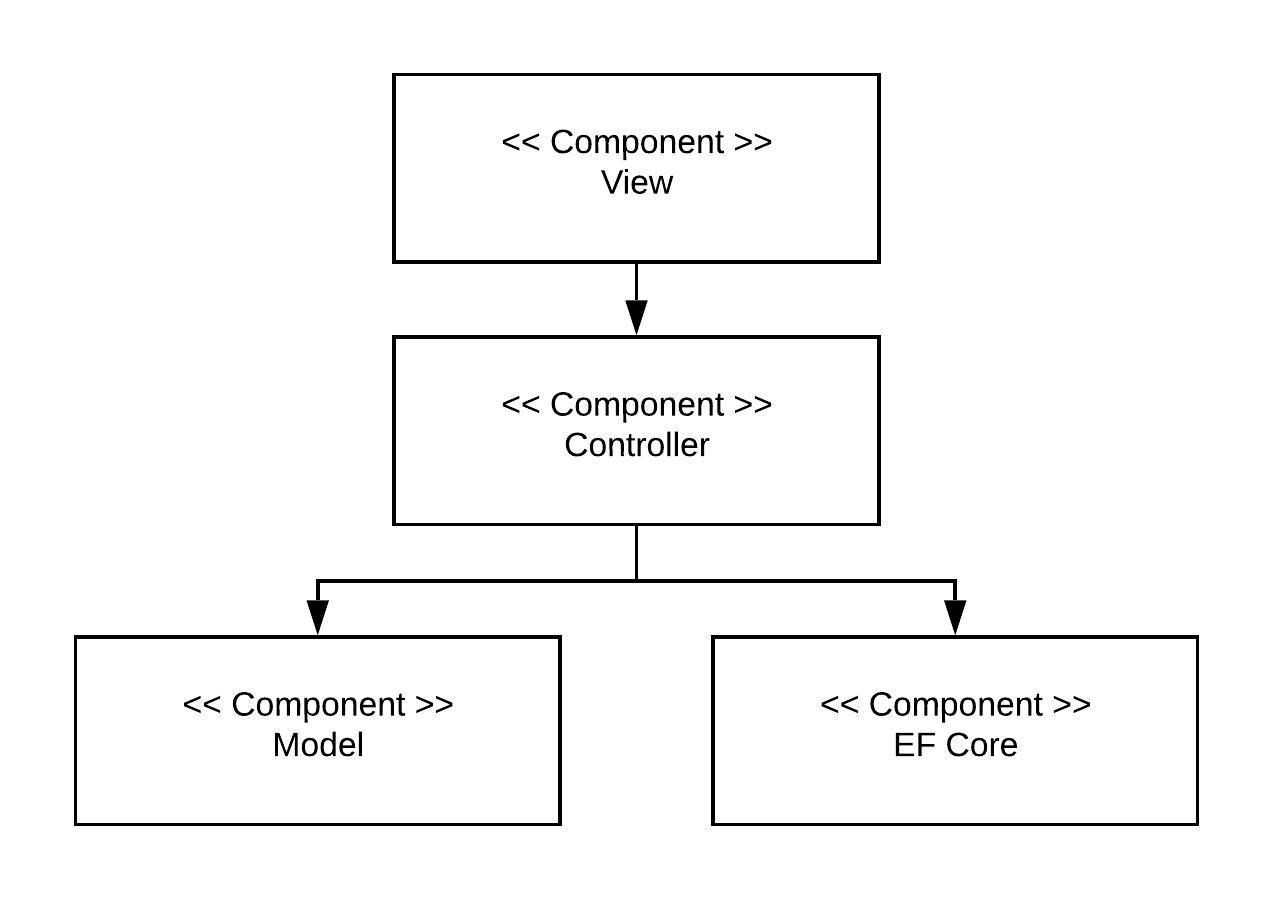
\includegraphics[width=0.7\textwidth]{billeder/simplecomponents.jpeg}
	\caption{Simple component layer design}\label{fig:SimpleComponent}
\end{figure}

View, controller, model, and EF Core are thus the main components layers that can be found in the design, each with a well-defined responsibility.
Ideally the architecture is designed so that the view and model components do not have to interact with each other.
% Kilde? Det virker lidt suspekt at views og models ikke skal kunne snakke med hinanden
% Anja: Virkelig? Tjah, saa tænker jeg slet sætningen ovenfor, da den er trukket ud af min røv
It is the intention that the controller is the link between these components, which is why it is placed in the middle of the layer components.
The main function of the controller is to link objects from the model component and data from the EF Core database and make these accessible for the view component.

%Anna: vil vove at påstå der ikke birde være et afsnit her
% Anja: Jeg vil paastaa det modsatte
This will not always be the case as the ASP.NET Core MVC model is designed so that a view has a corresponding controller.
For example the document view will have a corresponding document controller.
The document view will eventually have to borrow objects and data from other models in the system, which means that the view will at times have to bypass the controller component to communicate with the model component.

Subsystems can be explored from the main components, which e.g. are the interface system and its underlying technologies.
These are HTML, CSS, JavaScript and razor.
The model component has two main parts which are the model classes from the MVC pattern and the EF Core database system.
These two are defined as separate components which share similar responsibilities in the model component.
These components their relations with each other, and their underlying sub components can be seen in the complex version of the layer design below:

\begin{figure}[H]
	\centering
	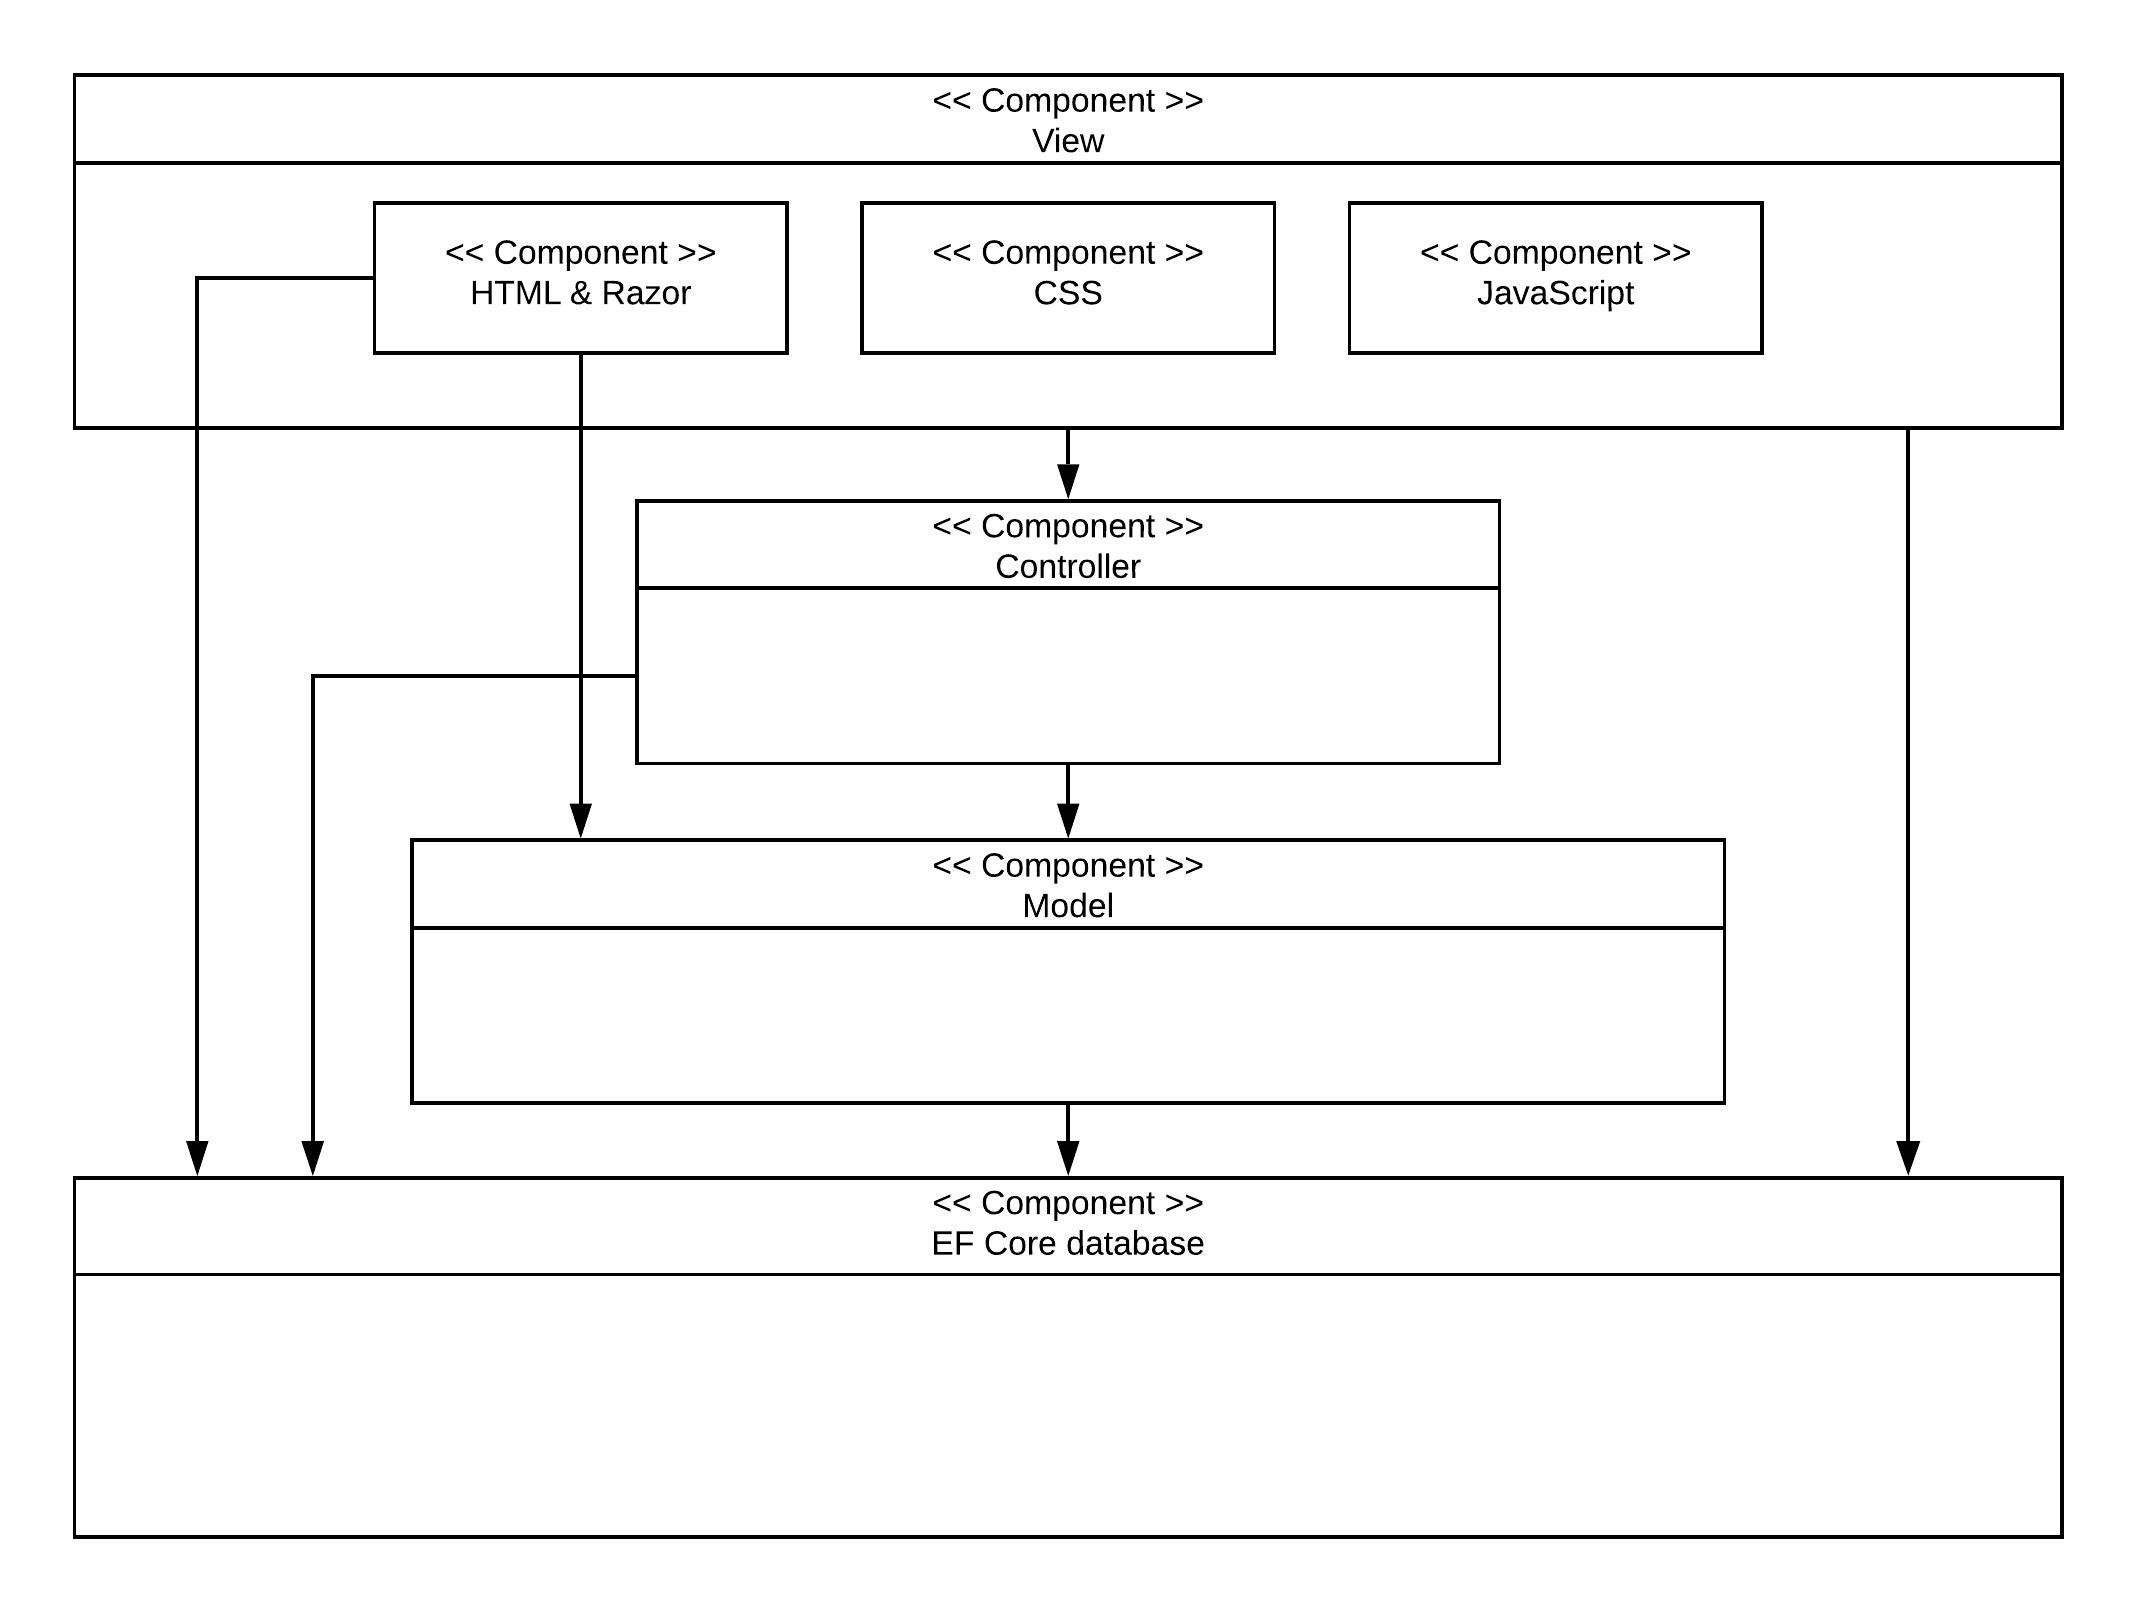
\includegraphics[width=1\textwidth]{billeder/complexcomponents.jpeg}
	\caption{Complex component layer design}
\end{figure}

Ideally the design would have \textit{closed-relaxed} architecture as the components would only be able to access layers adjacent to them.
In this design the design would be \textit{relaxed} as the controller would have access to both the view and the model components.
As it is though the design has an \textit{open-relaxed} architecture as the view component occasionally has access to the model component.
%Anna: Kan godt tænkes de to sidste sætninger trænger til en omskrivning
% Anja: Tjoh
% Henrik: Tænker at det er forkert med pil fra JavaScript til Model

In the final design there will be several classes included within each of the components.
Each of the main classes in the model component will have a corresponding controller and view in relation to it.
For example the document class in the model component will have a corresponding database in EF Core as well as a corresponding controller and view.
Here the documents object is within the model component and the documents data will be stored in the database.
A corresponding controller, which mainly handles the document class, ensures that the class and database are accessible for the actor.
The corresponding view ensures that the actor is able to see and interact with the document classes and database.

\section{Navigation Tree}
This section describes the navigation tree that visualizes how user move through the application, see \Cref{fig:Navigation}.
\begin{figure}
	\centering
	\begin{tikzpicture}[align=center, scale=1.0, transform shape]
		\node(login)[predefined]{Login};
		\node(activate)[predefined, right=0.4cm of login, yshift=0.7cm]{Activate\\account};
		\node(main)[predefined, right=0.4cm of activate, yshift=-0.7cm]{Main};
		
		\node(user-a)[predefined, right=0.4cm of main, yshift=-1.4cm]{User\\administration};
			\node(create)[predefined, right=0.4cm of user-a, yshift=0.7cm]{Create\\user};
			\node(user-i)[predefined, right=0.4cm of user-a, yshift=-0.7cm]{User\\info};
			\node(edit)[predefined, right=0.4cm of user-i]{Edit};
		\node(depart)[predefined, below=1.7cm of user-a]{Departments};
			\node(dep-detail)[predefined, right=0.4cm of depart]{Detail};
			\node(edit-U)[predefined, right=0.4cm of dep-detail, yshift=0.7cm]{Edit\\users};
			\node(edit-D)[predefined, right=0.4cm of dep-detail, yshift=-0.7cm]{Edit\\documents};
		\node(setting)[predefined, below=0.7cm of depart]{Settings};
		
		\node(archive)[predefined, right=0.6cm of main, yshift=1.0cm]{Archive};
			\node(preview)[predefined, right=0.6cm of archive]{Preview\\document};
		\node(approvals)[predefined, above=0.7cm of archive]{Approvals};
		\node(doc)[predefined, above=0.7cm of approvals]{Add new\\document};
		
		\node(fit)[draw=red, fit=(main) (edit-D) (doc) (setting)] {};
		\node(profile)[predefined, right=0.4cm of fit, yshift=0.7cm]{Edit\\profile};
		\node(out)[predefined, right=0.4cm of fit, yshift=-0.7cm]{Log\\out};
		
		\draw[black](login.east) -| (0.8,-0.7);
		\draw[black](0.8,-0.7) |- (activate.west);
		\draw[black](activate.east) -| (2.8,0.0);
		\draw[black](0.8,-0.7) -| (2.8,0.0);
		\draw[black](2.8,0.0) |- (main.west);
		\draw[black](main.east) -| (4.4,0.1);
		\draw[black](4.4,0.1) |- (doc.west);
		\draw[black](4.4,0.1) |- (approvals.west);
		\draw[black](4.4,0.1) |- (archive.west);
		\draw[black](main.east) -- (4.6,0.0);
		\draw[black](4.4,0.1) |- (user-a.west);
		\draw[black](4.4,0.1) |- (depart.west);
		\draw[black](4.4,0.1) |- (setting.west);
		\draw[black](6.7,0.5) |- (approvals.east);
		\draw[black](6.7,0.5) |- (archive.east);
		\draw[black](6.7,0.5) |- (4.6,0.0);
		\draw[black](6.7,0.5) |- (preview.west);
		\draw[black](7.6,-0.9) |- (user-a.east);
		\draw[black](7.6,-0.9) |- (user-i.west);
		\draw[black](7.6,-0.9) |- (create.west);
		\draw[black](user-i.east) |- (edit.west);
		\draw[black](depart.east) -- (dep-detail.west);
		\draw[black](dep-detail.east) -| (9.1,-3.5);
		\draw[black](edit-U.west) -| (9.1,-3.5);
		\draw[black](edit-D.west) -| (9.1,-3.5);
		\draw[black](fit.east)-| (11.7, 0.0);
		\draw[black](profile.west)-| (11.7, 0.0);
		\draw[black](out.west)-| (11.7, 0.0);
			
	\end{tikzpicture}
	\caption{Navigation tree}\label{fig:Navigation}
\end{figure}


The user will first encounter the Login page.
For the first-timer user they have to enter the Activate account page and insert the given username received from administrator to register email address (optional) and create a password.
Once activate account process is finished user will be redirected to the handbook's Main page.
If the account is already activated user will be redirected to the Main page once logged in.

In the Main page administrator and writer will be able to access the ``Add new document'' page.
Writer will be able to access awaiting approvals under the relevant document section in the Main page.
Administrator will be able to enter the Approvals page through a sidebar which is only accessible for administrator.
The sidebar consists of:

\begin{itemize}
	\item Handbook (return to the Main page)
	\item Approvals
	\item Archive
	\item User administration
	\item Departments
	\item Settings
\end{itemize}

The Preview document page can be access in three ways depends on access rights, see \Cref{tab:docPreviewEntries} below.

\begin{table}[H]
	\begin{center}
	\begin{tabular}{| m{20em} | c | c | c | c | c |}
		\hline
		Document preview entry & Administrator & Writer & Reader \\
		\hline
		 Directly through document in the valid handbook & x  & x & x\\
		\hline
		 Through archive document  & x &  & \\
		\hline
		 Via awaiting approval document & x & x &  \\
		\hline
	\end{tabular}
	\end{center}
	\caption{Document preview entries}\label{tab:docPreviewEntries}
\end{table}

Through the User administration page which is accessible from the sidebar administrator will be able to access the Create user page or the User info page to enter the Edit page and update user information.

Under the Departments page entered through the sidebar.
Administrator will be able to click on existing department name to enter the Detail page of an overview of associate users and documents.
In the Detail page administrator would be able to enter the Edit users page or the Edit documents page.

The Settings page is accessible from the sidebar where administrator can change the company name and enable or disabled changelog functionality to the application.

In the Navigation tree in \Cref{fig:Navigation} the red box indicate that every role can enter the Edit profile page or Log out on the global, top-level navigation bar anywhere in the navigation flow within the red box.

\end{document}
